% introduction.tex

\section{INTRODUCTION}

\subsection{Background of the Project}

    In response to persistent gaps in sponsorship billing and the growing demand for reliable financial records, this study proposes an integration first \textbf{SPONSOR MANAGEMENT AND LETTER OF GUARANTEE (LoG) COVERAGE INTEGRATION SYSTEM FOR INTERNATIONAL SCHOOL MANILA (ISM)}. The system recognizes sponsorship coverage as a common institutional reference rather than a local setup within a single application. Its architecture is based on a centralized Sponsor Master and a coverage rules engine, with uniform identifiers synchronized across  \textbf{PowerSchool} as the Student Information System (SIS) that stores the primary student profile,  \textbf{NetSuite} as the finance system that records student charges and maintains the student ledger, the in house  \textbf{Student Charging Portal} that processes student charges, and the  \textbf{Online Billing System} that displays statements of account for parents and sponsors. 
    
    International School Manila currently conducts student billing through these four systems, which were implemented at different points in time to satisfy specific operational requirements. \textbf{PowerSchool} holds enrollment and demographic records. Front line staff use the \textbf{Student Charging Portal} to create itemized charges. This is recorded in  \textbf{NetSuite} and included in the student ledger to be reported financially. These ledger entries are then presented as statements of account of parents and sponsors, which is displayed on the  \textbf{Online Billing System}.

    In this multi system setting, sponsorship billing is being facilitated by \textbf{Letters of Guarantee (LoG)} which are given by the sponsors stating the items or categories they will cover. When a charge entry is made in  \textbf{Student Charging Portal}, operators read and decode each LoG, and determine whether a line item is to be covered, and give the Bill To designation, either to a sponsor or to a parent. Such decisions are made by passing the chain of integration: the charges are entered into  \textbf{NetSuite} and the  \textbf{Online Billing System} reflects it in the statements of account that parents and sponsors see. Staff members use spreadsheet and comma separated value (CSV) files to manually match records across platforms to keep these systems synchronized.
    
    \begin{figure}
        \centering
        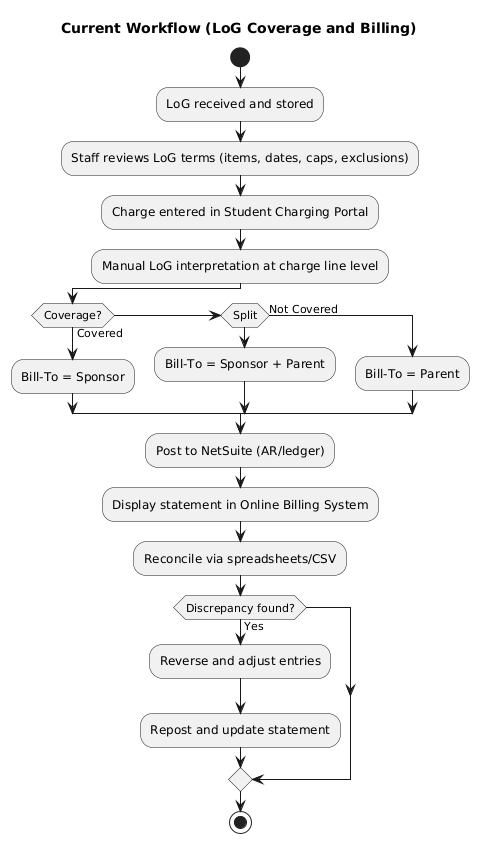
\includegraphics[width=0.75\linewidth]{Texfiles/images/Current Workflow.png}
        \caption{Current Workflow}
        \label{fig:Current Workflow}
    \end{figure}    
    
    This manual interpretation and file based reconciliation has over time shown some significant limitations. Spreadsheet parallel references and unofficial notes lose their connection to authoritative information. Staff are interpreting similar LoG provisions in different ways and thus providing different Bill To decisions on similar charges. Mispostings, late amendments, and missing documentation decrease confidence in the student ledger, complicate the reconciliation and put the institution at risk of audit and regulatory scrutiny. These problems are found within a regulatory environment that requires accuracy, openness, and accountability.
    
    ISM has to match student data in a third party SIS, billing capture in an in house portal, statements in an in house billing system, and accounting data in a third party finance platform and needs to follow the Bureau of Internal Revenue policy of the Ease of Paying Taxes (EoPT), which promotes well documented and clear billing records. A person dependent, fragmented vision of the sponsorship coverage in such context would impeccate more pressure on operations and governance. There are a number of other solutions but they pose serious trade offs to ISM.
    
    The first option is to implement a monolithic enterprise resource planning system which
    integrates student records, billing, ledgers and accounting to a single vendor system. Although this will minimize the number of applications, it will involve a massive migration of the system, renegotiation of the current integrations, and customization of school processes to vendor recommended workflow, which might not mirror the PowerSchool, NetSuite, and in house system combination that ISM has established.
    
    The second option is to implement specialized sponsorship management software or sponsor billing portals that are concerned with invoicing and collections. These tools tend to enhance payment tracking and usually still have manual interpretation at charge entry and rely on spreadsheets to reconcile, which leads to the same inconsistency in Bill To decisions.
    
    The third option is to keep enhancing the existing spreadsheet based process with tightening of the templates and more review control but this is also very much manual, person-based and is not easy to scale or audit. The proposed SPONSOR MANAGEMENT and LETTER of GUARANTEE (LoG) COVERAGE INTEGRATION SYSTEM in International School of Manila (ISM) is different than the other alternatives since it does not replace the existing core systems in the school but aims at and corrects the cause of inconsistency: the lack of a single, rule driven sponsorship coverage source.
    
    Instead of replacing PowerSchool, NetSuite, or the in house portals, the system positions the Sponsor Master and coverage rules engine as a shared institutional service that evaluates every charge in a consistent way. This allows line level, deterministic Bill To decisions to be returned at the moment of charge entry, carried forward into NetSuite as correctly posted transactions, and displayed in the Online Billing System as clear statements of account for parents and sponsors. In doing so, the proposal combines the strengths of the current landscape with centralized logic and explainable decisions, providing a more practical, lower risk, and institution specific solution than full system replacement or continued reliance on manual spreadsheets.

\subsection{DEFINITION OF TERMS}

    \begin{itemize}
  \item \textbf{AR:} Accounts Receivable
  \item \textbf{Azure:} Microsoft Azure, the cloud platform used to host system services and data
  \item \textbf{Bill To Designation:} Is the authoritative selection of the billing party for a charge line item, determining whether the sponsor, the parent, or both are assigned responsibility in downstream financial posting and statement presentation
  \item \textbf{BIR EoPT:} Bureau of Internal Revenue Ease of Paying Taxes
  \item \textbf{Cashier:} Staff who tag a student’s Sponsor in PS (SIS) using the sponsor drop-down sourced from the LoG system
  \item \textbf{Coverage Decision:} A deterministic evaluation outcome for a charge line item, classified as Covered, Split, or Not Covered, produced at the moment of charge entry and recorded with a reason code and rule version.
  \item \textbf{Coverage Evaluation:} The rule-based process that determines whether a sponsor covers a charge line item or category
  \item \textbf{Coverage Rule:} A deterministic rule that defines sponsor coverage by item or category, including limits, exceptions, and effective dates
  \item \textbf{CSV:} Comma-Separated Values, a flat-file format commonly used for data export and import
  \item \textbf{Deterministic rules engine:} Is a rules-based evaluation component that produces consistent coverage decisions from the same inputs by applying explicit rule priorities, constraints, and computation logic without predictive modeling.
  \item \textbf{ERP:} Enterprise Resource Planning
  \item \textbf{Identifier:} A unique reference value used to match and synchronize records across systems (for example, sponsor IDs and student IDs)
  \item \textbf{ISM:} International School Manila
  \item \textbf{IT Administrator:} Staff who configure integrations and schedules; under the target state, maintain sponsor records in the LoG system and monitor synchronization
  \item \textbf{Ledger:} The financial record of student charges and related transactions maintained within the finance system
  \item \textbf{Letter of Guarantee (LoG):} Is a sponsor-issued document that specifies the scope of charges the sponsor will cover, including limitations such as coverage caps, effective dates, exclusions, and required supporting documentation.
  \item \textbf{NetSuite:} The finance and accounting system used to record student charges and maintain the student ledger
  \item \textbf{NS (ERP):} NetSuite, the Enterprise Resource Planning system
  \item \textbf{OBS:} Online Billing System
  \item \textbf{Online Billing System:} The system that displays statements of account to parents and sponsors
  \item \textbf{PowerSchool:} The Student Information System (SIS) used to store primary student enrollment and profile data
  \item \textbf{PS (SIS):} PowerSchool, the Student Information System
  \item \textbf{Reason Code:} A machine readable label that explains a coverage or billing decision
  \item \textbf{Rules Engine:} The software component that applies coverage rules to charge entries and produces consistent, explainable outcomes
  \item \textbf{SCP:} Student Charging Portal
  \item \textbf{SCP Operator:} Staff who enter student charges in SCP and rely on the coverage decision
  \item \textbf{SIS:} Student Information System
  \item \textbf{Sponsor:} Refers to an external organization, agency, or individual that assumes full or partial financial responsibility for a student’s assessed charges based on an approved Letter of Guarantee (LoG). Sponsorship is operationalized as a rule-governed billing relationship that defines covered charge items or categories, coverage limits, effective dates, exclusions, required documentation, and allocation terms between sponsor and parent responsibility.
  \item \textbf{Sponsor–parent allocation:} Allocation is the computed distribution of a charge amount across sponsor and parent responsibility, expressed as amounts and, when applicable, percentages.
  \item \textbf{Sponsor Master:} Is the canonical repository of sponsor identities, attributes, identifiers, and governance controls used to synchronize consistent sponsor records across PowerSchool, the Student Charging Portal, NetSuite, and the Online Billing System.
  \item \textbf{SponsorID:} Canonical unique identifier for a sponsor in this system
  \item \textbf{Statement of Account (SOA):} An itemized billing statement showing charges and the allocation of responsibility between sponsor and parent
  \item \textbf{Student Charging Portal:} The in-house system used by staff to create and submit itemized student charges
  \item \textbf{Transaction:} A recorded financial event, such as a charge entry, that is posted to the finance system and reflected in billing statements
\end{itemize}

\subsection{OBJECTIVES}

\subsubsection{General Objective}

    To design and develop an integrated SPONSOR MANAGEMENT AND LETTER OF GUARANTEE (LoG) COVERAGE INTEGRATION SYSTEM FOR INTERNATIONAL SCHOOL MANILA (ISM) that automates sponsor management and Letter of Guarantee coverage validation across PowerSchool, NetSuite, the Student Charging Portal, and the Online Billing System.

\subsubsection{Specific Objectives}

    \begin{enumerate}
    \item To synchronize and combine the sponsor management and coverage validation between PowerSchool, NetSuite, the Student Charging Portal and the Online Billing System through authoring and maintaining similar identifiers, updates being made based on business events such as create, update and merge.
    \item To achieve real time, explainable coverage evaluation in the Student Charging Portal based on a deterministic rules engine, which implements sponsor coverage rules on entry of charge and provides human readable reason codes on Bill To determinations.
    \item To create a centralized Sponsor Master that keeps canonical records of sponsor data, such as sponsor data, coverage policies, limits, and effective dates, and status and provides the identifiers needed to tag students and record financial transactions in PowerSchool and NetSuite.
    \item To make sure that the correct Bill To designation is set up in NetSuite and the Online 
    Billing System so that it can be complied with and audited, to produce documentation that satisfies the BIR Ease of Paying Taxes requirements, and to record correct sponsor-parent allocations to the student ledger and the general ledger.
    \item To enforce data quality and governance within the Sponsor Master through validation of required fields and classification attributes, duplicate detection and merge workflows, and maintenance of authoritative cross system identifiers.
    \end{enumerate}

\subsection{SCOPE}

    The project covers the analysis, design, and prototype implementation of the SPONSOR MANAGEMENT AND LETTER OF GUARANTEE (LoG) COVERAGE INTEGRATION SYSTEM FOR INTERNATIONAL SCHOOL MANILA (ISM) hosted on Microsoft Azure. It includes the design and deployment of the Sponsor Master repository that stores sponsor records, coverage attributes, and cross system identifiers, as well as the development of a rules model for item and category level coverage with limits and defined exceptions.
    
    The scope further includes implementation of real time coverage evaluation within the Student Charging Portal, propagation of coverage decisions to NetSuite for posting and maintenance of the student ledger, and synchronized presentation of covered and non covered items in the Online Billing System as statements of account for parents and sponsors. Statements will show sponsor and parent responsibility, the governing rule, and relevant metadata. Primary users include Cashiers and Student Charging Portal operators, Finance and Accounting staff in NetSuite, and authorized administrators at the department and school level, with parents and sponsors viewing statements through the Online Billing System.
    
    The project focuses on core integration flows, coverage evaluation logic, essential user interface components needed to test coverage preview and explanations in the Student Charging Portal, and control and logging mechanisms that support review of sponsor related transactions.

\subsection{LIMITATIONS}

    The initial phase of the SPONSOR MANAGEMENT AND LETTER OF GUARANTEE (LoG) COVERAGE INTEGRATION SYSTEM FOR INTERNATIONAL SCHOOL MANILA (ISM) is limited to a functional prototype and does not extend to full production hardening. The work focuses on integration and coverage evaluation and does not include predictive analytics, financial forecasting, or optimization of sponsor portfolios. Comprehensive user interface redesign for PowerSchool, NetSuite, or the Online Billing System is outside the scope; these systems are expected to retain their existing interfaces, with only targeted enhancements to surface coverage related information.
    
    Integration depends on the application programming interfaces and secure file based exchanges supported by PowerSchool, NetSuite, and the in house systems. Constraints in these interfaces may limit real time synchronization and may require scheduled or batched updates for some data sets. Historical sponsor records and retroactive restatement of past sponsorship decisions are not included. Validation will rely on representative, deidentified data and structured user acceptance testing aligned with current Letters of Guarantee. 
    
    Performance tuning, advanced monitoring, disaster recovery, and high availability will be addressed only to the level appropriate for a prototype, and further work will be required before production deployment. The project does not include changes to tuition policy, contractual terms with sponsors, or fundamental business rules beyond those needed to encode existing coverage agreements into the rules engine and the Sponsor Master.
    